\documentclass[letterpaper]{article} % DO NOT CHANGE THIS
\usepackage[submission]{aaai24}  % DO NOT CHANGE THIS
\usepackage{times}  % DO NOT CHANGE THIS
\usepackage{helvet}  % DO NOT CHANGE THIS
\usepackage{courier}  % DO NOT CHANGE THIS
\usepackage[hyphens]{url}  % DO NOT CHANGE THIS
\usepackage{graphicx} % DO NOT CHANGE THIS
\urlstyle{rm} % DO NOT CHANGE THIS
\def\UrlFont{\rm}  % DO NOT CHANGE THIS
\usepackage{natbib}  % DO NOT CHANGE THIS AND DO NOT ADD ANY OPTIONS TO IT
\usepackage{caption} % DO NOT CHANGE THIS AND DO NOT ADD ANY OPTIONS TO IT
\frenchspacing  % DO NOT CHANGE THIS
\setlength{\pdfpagewidth}{8.5in} % DO NOT CHANGE THIS
\setlength{\pdfpageheight}{11in} % DO NOT CHANGE THIS
%
% These are recommended to typeset algorithms but not required. See the subsubsection on algorithms. Remove them if you don't have algorithms in your paper.
\usepackage{algorithm}
\usepackage{algorithmic}

%
% These are are recommended to typeset listings but not required. See the subsubsection on listing. Remove this block if you don't have listings in your paper.
\usepackage{newfloat}
\usepackage{listings}

% User imported packages
\usepackage{multirow}
\usepackage{pifont}
\usepackage{booktabs}
\usepackage{subcaption}
\usepackage{bm}
\usepackage{amsmath}
\usepackage{amssymb}
\usepackage{cleveref}
\usepackage{todonotes}
\usepackage{varwidth}
\usepackage{tikz}
\usepackage{graphicx}
\newcommand{\cmark}{\ding{51}} % checkmark symbol
\newcommand{\xmark}{\ding{55}} % X-mark symbol

\DeclareCaptionStyle{ruled}{labelfont=normalfont,labelsep=colon,strut=off} % DO NOT CHANGE THIS
\lstset{%
	basicstyle={\footnotesize\ttfamily},% footnotesize acceptable for monospace
	numbers=left,numberstyle=\footnotesize,xleftmargin=2em,% show line numbers, remove this entire line if you don't want the numbers.
	aboveskip=0pt,belowskip=0pt,%
	showstringspaces=false,tabsize=2,breaklines=true}
\floatstyle{ruled}
\newfloat{listing}{tb}{lst}{}
\floatname{listing}{Listing}
%
% Keep the \pdfinfo as shown here. There's no need
% for you to add the /Title and /Author tags.
\pdfinfo{
/TemplateVersion (2024.1)
}

% DISALLOWED PACKAGES
% \usepackage{authblk} -- This package is specifically forbidden
% \usepackage{balance} -- This package is specifically forbidden
% \usepackage{color (if used in text)
% \usepackage{CJK} -- This package is specifically forbidden
% \usepackage{float} -- This package is specifically forbidden
% \usepackage{flushend} -- This package is specifically forbidden
% \usepackage{fontenc} -- This package is specifically forbidden
% \usepackage{fullpage} -- This package is specifically forbidden
% \usepackage{geometry} -- This package is specifically forbidden
% \usepackage{grffile} -- This package is specifically forbidden
% \usepackage{hyperref} -- This package is specifically forbidden
% \usepackage{navigator} -- This package is specifically forbidden
% (or any other package that embeds links such as navigator or hyperref)
% \indentfirst} -- This package is specifically forbidden
% \layout} -- This package is specifically forbidden
% \multicol} -- This package is specifically forbidden
% \nameref} -- This package is specifically forbidden
% \usepackage{savetrees} -- This package is specifically forbidden
% \usepackage{setspace} -- This package is specifically forbidden
% \usepackage{stfloats} -- This package is specifically forbidden
% \usepackage{tabu} -- This package is specifically forbidden
% \usepackage{titlesec} -- This package is specifically forbidden
% \usepackage{tocbibind} -- This package is specifically forbidden
% \usepackage{ulem} -- This package is specifically forbidden
% \usepackage{wrapfig} -- This package is specifically forbidden
% DISALLOWED COMMANDS
% \nocopyright -- Your paper will not be published if you use this command
% \addtolength -- This command may not be used
% \balance -- This command may not be used
% \baselinestretch -- Your paper will not be published if you use this command
% \clearpage -- No page breaks of any kind may be used for the final version of your paper
% \columnsep -- This command may not be used
% \newpage -- No page breaks of any kind may be used for the final version of your paper
% \pagebreak -- No page breaks of any kind may be used for the final version of your paperr
% \pagestyle -- This command may not be used
% \tiny -- This is not an acceptable font size.
% \vspace{- -- No negative value may be used in proximity of a caption, figure, table, section, subsection, subsubsection, or reference
% \vskip{- -- No negative value may be used to alter spacing above or below a caption, figure, table, section, subsection, subsubsection, or reference

\setcounter{secnumdepth}{0} %May be changed to 1 or 2 if section numbers are desired.

% The file aaai24.sty is the style file for AAAI Press
% proceedings, working notes, and technical reports.
%

% Title

% Your title must be in mixed case, not sentence case.
% That means all verbs (including short verbs like be, is, using,and go),
% nouns, adverbs, adjectives should be capitalized, including both words in hyphenated terms, while
% articles, conjunctions, and prepositions are lower case unless they
% directly follow a colon or long dash
\iffalse\title{AAAI Press Anonymous Submission\\Instructions for Authors Using \LaTeX{}}
\author{
    %Authors
    % All authors must be in the same font size and format.
    Written by AAAI Press Staff\textsuperscript{\rm 1}\thanks{With help from the AAAI Publications Committee.}\\
    AAAI Style Contributions by Pater Patel Schneider,
    Sunil Issar,\\
    J. Scott Penberthy,
    George Ferguson,
    Hans Guesgen,
    Francisco Cruz\equalcontrib,
    Marc Pujol-Gonzalez\equalcontrib}
\affiliations{
    %Afiliations
    \textsuperscript{\rm 1}Association for the Advancement of Artificial Intelligence\\
    % If you have multiple authors and multiple affiliations
    % use superscripts in text and roman font to identify them.
    % For example,

    % Sunil Issar\textsuperscript{\rm 2},
    % J. Scott Penberthy\textsuperscript{\rm 3},
    % George Ferguson\textsuperscript{\rm 4},
    % Hans Guesgen\textsuperscript{\rm 5}
    % Note that the comma should be placed after the superscript

    1900 Embarcadero Road, Suite 101\\
    Palo Alto, California 94303-3310 USA\\
    % email address must be in roman text type, not monospace or sans serif
    proceedings-questions@aaai.org
%
% See more examples next
}
\fi

%Example, Single Author, ->> remove \iffalse,\fi and place them surrounding AAAI title to use it
\iffalse\title{My Publication Title --- Single Author}
\author{
    Author Name
}
\affiliations{
    Affiliation\\
    Affiliation Line 2\\
    name@example.com
}
\fi

%Example, Multiple Authors, ->> remove \iffalse,\fi and place them surrounding AAAI title to use it
\title{Learning Rate Optimization for Online Deep Learning}
\author{
    % Authors
    Lucas Cazzonelli\textsuperscript{\rm 1},
    Cedric Kulbach\textsuperscript{\rm 2},
}
\affiliations{
    % Affiliations
    \textsuperscript{\rm 1}FZI Research Center for Information Technology\\
    \textsuperscript{\rm 2}Affiliation 2\\
    cazzonelli@fzi.de, secondAuthor@affilation2.com
}


% REMOVE THIS: bibentry
% This is only needed to show inline citations in the guidelines document. You should not need it and can safely delete it.
\usepackage{bibentry}
% END REMOVE bibentry

\begin{document}

\maketitle


\begin{abstract}

	\noindent Efficient training via gradient-based optimization techniques is an essential building block to the success of deep learning. Extensive research on the impact and the effective estimation of an appropriate learning rate has partly enabled these techniques. Despite the proliferation of data streams generated by IoT devices, digital platforms, etc., previous research has been primarily focused on batch learning, which assumes that all training data is available a priori. However, characteristics such as the gradual emergence and non-stationarity of data pose additional challenges. Therefore, the findings on batch learning may not be applicable to deep learning in streaming environments. In this work, we seek to address this knowledge gap by (i) evaluating and comparing typical learning rate schedules and optimizers, (ii) exploring adaptations of these techniques, and (iii) providing insights into effective learning rate tuning in the context of stream-based deep learning.


\end{abstract}

\section{Introduction}
Deep learning models have demonstrated exceptional performance in various domains, with the choice of optimizer playing a crucial role in achieving outstanding results.
In the context of batch learning, where all data is available at a time, extensive research has been conducted to explore optimization techniques for deep learning architectures and numerous methods have emerged to effectively update the weights of these architectures.
Further, the recent development of deep learning frameworks for online learning scenarios foster the application and the research of deep learning models in dynamic scenarios such as on data streams. 
However, with the application of deep learning models on data streams new challenges arise, as data streams evolve over time the models are affected by potential changes in the underlying data structure, that is also referred to as concept drift. 
In order to achieve high predictive performance and a fast adaptation of the networks weights to new data patterns a suitable choice of the underlying optimizer becomes crucial.
This paper aims to bridge this knowledge gap by investigating how the choice of optimizer changes when transitioning from batch learning to online learning scenarios and discusses different optimization strategies when applying deep learning models in online learning scenarios.
Specifically, we address the following research questions:
\begin{enumerate}
	\item How does the choice for the optimizer change from batch to online learning?
	\item What are practical choices for gradient-based online training of deep architectures in online learning?
	\item Are adaptive optimization methods better suited in Online Deep Learning?
\end{enumerate}


\todo{Online Learning Req. in Kontext einbetten!}
% In contrast to conventional batch learning, the impact of the learning rate in stream-based deep learning is a lesser studied issue.
According to \citet{bifetMOAMassiveOnline2010} a machine learning model operating in such an environment must be able to
\begin{center}
	\begin{varwidth}{0.5\textwidth}
		\begin{description}
			\item[R1:] process a single instance at a time,\label{rq:single_instance}
			\item[R2:] process each instance in a limited amount of time,\label{rq:limited_time}
			\item[R3:] use a limited amount of memory,\label{rq:limited_memory}
			\item[R4:] predict at any time,\label{rq:predict_any_time}
			\item[R5:] adapt to changes in the data distribution.\label{rq:adapt_to_drift}
		\end{description}
	\end{varwidth}
\end{center}

\todo{Put LR tuning graphic here?}
\begin{figure}[ht]
	\centering
	\begin{tikzpicture}
		% Upper image
		\node[inner sep=0pt] (upper) {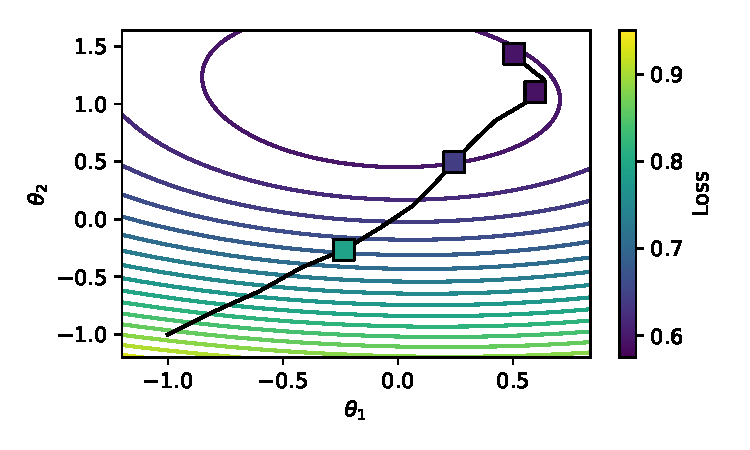
\includegraphics[width=0.4\textwidth]{figures/adam_trajectory_drift_reset1.pdf}};

		% Lower image
		\node[inner sep=0pt, below=3mm of upper] (lower){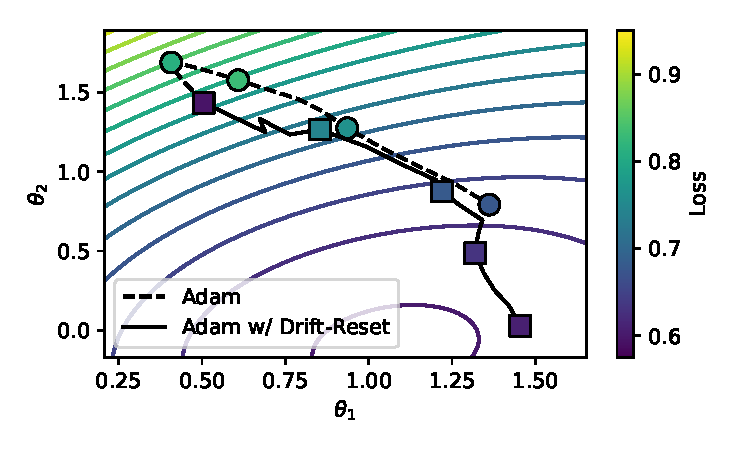
\includegraphics[width=0.4\textwidth]{figures/adam_trajectory_drift_reset2.pdf}};

		\path ([xshift=-8pt]upper) -- ([xshift=-8pt]lower) node[midway] (text){Concept Drift};
		\draw[->] ([xshift=-5pt, yshift=5pt]upper.south-|text.west) -- ([xshift=-5pt, yshift=-3pt]lower.north-|text.west);
		\draw[->] ([xshift=5pt, yshift=5pt]upper.south-|text.east) -- ([xshift=5pt, yshift=-3pt]lower.north-|text.east);

	\end{tikzpicture}
	\caption{Parameter trajectory of Adam~\cite{kingmaAdamMethodStochastic2017b} with or without drift adaptation on synthetic data stream with abrupt concept drift. Marker colors depict the expected prequential loss over the last 16 data instances.}
\end{figure}

\section{Learning Rate in First Order Stochastic Optimization}

In the following, we will explain the theoretical background of first-order stochastic optimization enabling modern deep learning models.
We will also outline the differences between the application of these techniques in traditional batch learning and online learning in terms of impact of the learning rate and its optimization.

First-order stochastic optimization algorithms like stochastic gradient descent typically aim to solve
\begin{equation}
	\min_{\theta} \mathbb{E}_{x \sim p(x)} [\mathcal{L}(x, \theta)],
\end{equation}
where $\mathcal{L}(x, \theta)$ represents a loss function that quantifies the predictive error of the model given a mini-batch of data samples $x$ and model parameters $\theta$.
The blueprint process of solving this problem via first order stochastic optimization consists of the following steps for each iteration $t \in 0, \ldots, T$:
\begin{enumerate}
	\item Draw a mini-batch of samples $x_t$ from distribution $p(x)$.
	\item Calculate the loss $\mathcal{L}_t = \mathcal{L}(x_t, \theta_t)$ for $x_t$ and current parameters $\theta_t$.
	\item Compute the gradient $g_t = \nabla_{\theta_t} \mathcal{L}_t$ with respect to the parameters.
	\item Update the parameters for the next iteration using $g_t$ and potentially information from past iterations.
\end{enumerate}

For basic SGD, we can define the parameter update performed at the end of each iteration as
\begin{equation}
	\theta_{t}  = \theta_{t} - \eta_t \cdot g_t,
\end{equation}
where $\eta_t$ denotes the step size or \textit{learning rate} at timestep $t$.

As previously described, the learning rate has an immense impact on the performance of the optimization process and therefore on the performance of a deep learning model as a whole.

The primary trade-off to consider with respect to the choice of $\eta$ is that increasing the learning rate speeds up convergence, but at the same time also increases stochasticity and therefore leads to the divergence of the training criterion beyond a certain threshold.~\cite{bengioPracticalRecommendationsGradientbased2012}.
In fact, \citet{smithBayesianPerspectiveGeneralization2018}, found that when modelling SGD as a stochastic differential equation, the “noise scale” is directly tied to $\eta$~\cite{smithBayesianPerspectiveGeneralization2018}.
In biological terms, increasing the learning rate increases plasticity, whereas decreasing it increases stability.
% Maybe remove? I like the biological analogy, but its usually used to describe plasticity and stability w.r.t. forgetting.

\subsection{Learning Rate Schedules}

While using a single fixed learning rate $\eta_t = \eta$ for all iterations simplifies the learning selection and can often yield sufficient performance, results can generally be improved with a schedule with step sizes specific to each iteration~\cite{wuDemystifyingLearningRate2019b}. 
To ensure fast convergence at the start of training, while mitigating jumping around potential minima at later stages it is, for instance, common to use a decaying schedule starting with a large learning rate that decreases over time.
An additional benefit of this approach is that of potentially better generalization, since larger learning rates can help skipping over sharp minima with poor generalization~\cite{hochreiterFlatMinima1997,chaudhariEntropySGDBiasingGradient2017}.
Some have likened this procedure to simulated annealing, which shifts its focus from exploration at high temperatures to exploitation once temperatures have sufficiently decreased~\cite{smithDonDecayLearning2018}.

A commonly used forms of decay are exponential decay, where $\eta_{t}$ calculates as
\begin{equation}
	\eta_{t} = \eta_0 \cdot \gamma^t,
\end{equation}
with $\gamma < 1$, and stepwise decay, which for a regular interval between steps of length $s$ is given as
\begin{equation}
	\eta_{t} = \eta_0 \cdot \gamma^{\lfloor t/s \rfloor}.
\end{equation}

Other popular options include cyclic learning rate schedules which oscillate $\eta$ between two values over a predefined interval.
For a basic triangular cycle, the learning rate calculates as
\begin{equation}
	\eta_t = \eta_0 + \frac{\hat{\eta} - \eta_0}{2s} \cdot \min_{i} \{|t-i\cdot s|\},
\end{equation}
with $\hat{\eta}$ being the learning rate at the middle of each cycle of length $s$.
Some studies~\cite{smithCyclicalLearningRates2017, smithSuperConvergenceVeryFast2018a} have found cyclic schedules to significantly speed up the convergence of neural networks even when compared to adaptive techniques like Adam in some cases~\cite{kingmaAdamMethodStochastic2017b}.
While there are many other learning rate schedules, we focus on the use of the three aforementioned schedules within data streaming applications in this work.
For a comprehensive overview and detailed analysis on learning rate policies, we refer to \citet{wuDemystifyingLearningRate2019b}.

\subsection{Adaptive Learning Rates}

While determining the learning rate through a separate tuning phase with parameter searches like grid- or random-search is still the de facto standard in deep learning~\cite{defazioLearningRateFreeLearningDAdaptation2023a}, this approach causes significant computational overhead.

To reduce this overhead, several previous works have developed \textit{adaptive optimizers}, which adjust the learning rate based on additional information about the loss landscape obtained from previous gradients at each optimization step, increasing the robustness with respect to the step size~\cite{duchiAdaptiveSubgradientMethods2011}.

One of the earlier optimizers in this category is \textit{AdaGrad}~\cite{duchiAdaptiveSubgradientMethods2011}, which divides the learning rate by the square root of the uncentered total sum of squares over all previous gradients, for each model parameter resulting in a parameter specific learning rate.
Unlike a single global value, parameter specific learning rates therefore not only influence the length, but also the direction of update steps, in case of AdaGrad by shifting updates in the direction of smaller gradients~\cite{wuWNGradLearnLearning2020}. % Weglassen? 

Among several other approaches like AdaDelta~\cite[see e.g.]{zeilerADADELTAAdaptiveLearning2012a} and RMSProp~\cite{tielemanLecture5rmspropDivide2012}, \citet{kingmaAdamMethodStochastic2017b} subsequently introduced Adam as an extension of AdaGrad, that additionally takes a momentum term of past gradients into account~\cite[see]{sutskeverImportanceInitializationMomentum2013} to speed up the convergence for parameters with consistent gradients.

While adaptive approaches such as AdaGrad and Adam have been shown to reduce the dependence on the learning rate, they often times still require manual tuning~\cite{wuWNGradLearnLearning2020}.
A problem that parameter-free variants of SGD aim to solve by estimating the optimal step size online as training progresses, thus eliminating the learning rate altogether.

For instance, \citet{schaulNoMorePesky2013} proposed \textit{vSGD}, which, like Adam, uses first and second order moments of the gradients as well as local curvature information to estimate $\eta$~\cite{schaulNoMorePesky2013}.
The authors obtain the latter by estimating positive diagonal entries of the Hessian with respect to the parameters through a back-propagation formula~\cite{schaulNoMorePesky2013}.
Even though \citet{schaulNoMorePesky2013} demonstrate \textit{vSGD's} robustness to non-stationary data distributions, it has, to the best of our knowledge, not been widely adopted in the online learning space.
Due to the lack of publicly available implementations of the non-trivial algorithm, we have not been able to evaluate vSGD at the time of writing. \todo{Did not evaluate vSGD since its old and there is no implementation. Is that valid?}

Instead of using curvature information for adapting $\eta$, the \textit{COCOB} algorithm proposed by~\citet{orabonaTrainingDeepNetworks2017} models parameter optimization as a gambling problem, in which the goal is to maximize the rewards obtained from betting on each gradient.
The model parameters are then computed based on the rewards accumulated over all previous timesteps~\cite{orabonaTrainingDeepNetworks2017}.
Intuitively, this corresponds to running a meta optimization algorithm, that estimates the expected optimal learning rate in parallel with the actual parameter optimization process.

Similar 

-Hypergradient Descent \cite{baydinOnlineLearningRate2018}: optimizes the learning rate of stochastic optimizers like SGD using a meta-gradient descent procedure.
-WNGrad \cite{wuWNGradLearnLearning2020}: adapts the dynamic update of AdaGrad to a single learning rate.

Another popular fram
In OCO literature it is well known that under the assumption of convexity of the loss function w.r.t. $\theta$, the worst-case optimal fixed learning rate is
\begin{equation}
	\eta^* = \frac{\theta^* - \theta_0}{\sqrt{\sum_{t=0}^{T} ||g_t||^2}},
\end{equation}

-Mechanic \cite{cutkoskyMechanicLearningRate2023}: can wrap around any first order algorithm, removing the need of tuning $\eta$. Uses a base online convex optimization algorithm as well as a meta OCO algorithm to optimize the learning rate with respect to the theoretical upper convergence bound of SGD
-DoG \cite{ivgiDoGSGDBest2023}: also optimizes theoretical upper bound by estimating $||\theta_0 - \theta^*||$ as $\max_{i<t}||\theta_0 - \theta_i||$
-D-Adaptation~\cite{defazioLearningRateFreeLearningDAdaptation2023a}: can modify popular optimizers by estimating $D$ with weighted dual averaging~\cite{duchiDualAveragingDistributed2012}


Furthermore, several studies developed parameter-free optimizers for specific areas of application such as time series forecasting~\cite{miyaguchiCograConceptDriftAwareStochastic2019,fekriDeepLearningLoad2021, zhangPOLAOnlineTime2021a}, federated learning~\cite{canonacoAdaptiveFederatedLearning2021} and recommender systems~\cite{ferreirajoseADADRIFTAdaptiveLearning2020}.
Due to our focus for the present work being general data stream applications, we did not further investigate these techniques.

Despite the fact that parameter-free stochastic optimization techniques are inherently well-suited for the highly non-stationary streaming data~\cite{schaulNoMorePesky2013} and in some cases even developed based on online convex optimization, their application on this kind of data has rarely been investigated.
This raises the question, whether they are suitable for stream-based learning (ii).


\begin{table}[ht]
	\centering
	\small
	\begin{tabular}{@{}lllcc@{}}
		\toprule
		Optimizer & Runtime                         & Space             & Param. specific & LR free \\ \midrule
		DAdapt    & $\mathcal{O}(6D)$               & $\mathcal{O}(2D)$ & \xmark          & \cmark  \\
		DoG       & $\mathcal{O}(5D)$               & $\mathcal{O}(1D)$ & \xmark          & \cmark  \\
		Mechanic  & $\mathcal{O}(10D)$              & $\mathcal{O}(1D)$ & \xmark          & \cmark  \\
		WNGrad    & $\mathcal{O}(2D)$               & $\mathcal{O}(0)$  & \xmark          & \cmark  \\
		SGDHD     & $\mathcal{O}(2D)$               & $\mathcal{O}(1D)$ & \xmark          & \cmark  \\
		COCOB     & $\mathcal{O}(14D)$              & $\mathcal{O}(4D)$ & \cmark          & \cmark  \\
		Adam      & $\mathcal{O}(12D)$              & $\mathcal{O}(2D)$ & \cmark          & \xmark  \\
		vSGD      & $\mathcal{O}(21D)$\footnotemark & $\mathcal{O}(4D)$ & \cmark          & \cmark  \\ % Remove since not evaluated?
		AdaGrad   & $\mathcal{O}(5D)$               & $\mathcal{O}(1D)$ & \cmark          & \xmark  \\ \bottomrule
	\end{tabular}
	\caption{Overview of additional time- and space-complexity of adaptive first-order optimizers compared to basic SGD. Values are given in big O notation with respect to the number of model parameters $D$. We do not list convergence guarantees because the guarantees given in the original papers of different optimizers are based on different assumptions and are rarely compatible with streaming applications.}\label{tab:param_free_optims}
\end{table}
\footnotetext[1]{Complexity for feed-forward neural networks. Since \textit{vSGD} requires additional backpropagation steps, its complexity is architecture dependent.}

\section{Differences between Batch and Online Learning}

In a batch learning setting, optimizing the learning rate comes down to finding values that minimize the expected loss on a hold-out set of validation data at the end of the training process.
Formally, we can denote this task as
\begin{equation}
	\label{eq:batch_lr_optim}
	\min_{\eta_0, \ldots, \eta_T} \mathbb{E}_{x \sim p_v(x)}[\mathcal{L}(x, \theta_T)],
\end{equation}
where $p_v$ is a distribution of held-out validation data and $\theta_T$ the parameters at the end of training, which for basic SGD are given by
\begin{equation}
	\theta_T = \sum_{t=0}^{T} \eta_t \cdot g_t.
\end{equation}

In online learning where data is generated incrementally, this notion of learning rate optimization is infeasible.
Due to requirements \textbf{RQ1-RQ5} models operating in an online streaming environment must be evaluated in a \textit{prequential} manner~\cite{bifetMOAMassiveOnline2010}, where each instance $x_t$ in the data stream is first used to test and then to train the model ensuring that testing is done exclusively on unseen data.

Training in such a scenario can therefore be more accurately modeled as an \textit{online convex optimization} (OCO) problem~\cite{shalev-shwartzOnlineLearningOnline2011,hazanIntroductionOnlineConvex2016}, where the optimizer suffers a loss $\mathcal{L}_t(\theta_t) = \mathcal{L}(x_t, \theta_{t})$ and produces updated parameters $\theta_{t+1}$ at each iteration of the data stream.

The task of finding an optimal learning rate schedule in this setting, can be formulated as
\begin{equation}
	\label{eq:stream_lr_optim}
	\min_{\eta_0, \ldots, \eta_T} \sum_{t=0}^{T} \mathcal{L}(x_t, \theta_t),
\end{equation}
where data samples $x_t$ are drawn from a distribution $p_t(x)$.

Compared to Problem~\eqref{eq:batch_lr_optim}, Problem~\eqref{eq:stream_lr_optim} features some key differences.
Due to Requirement~\ref{rq:predict_any_time}, the goal is to minimize the total sum of losses incurred over all timesteps of the prequential evaluation process,  instead of minimizing the only the validation loss for the final parameters $\theta_T$.
This means that not only the loss achieved by the final parameters $\theta_T$, but the loss suffered at every timestep of the stream contributes equally to the objective.
Therefore, speed of convergence is of larger importance in the streaming setting, whereas the performance of the final parameters $\theta_T$ has relatively little impact.
Since memory is limited (Requirement~\ref{rq:limited_memory}), it is also not possible to continue training on previously observed data as long as $\mathcal{L}$ decreases, which puts an even greater emphasis on quick adaptation.
At the same time, a larger learning rate causing temporary loss increases, due to skipping over local minima can be suboptimal with respect to Problem~\ref{eq:stream_lr_optim} even if it eventually yields a lower loss.

Another difference to conventional batch learning is that the distribution $p_t$ is time dependent, due to the fact that data streams might, and in practice most likely will, be subjected to change in the form of \textit{concept drift}\footnote{We use concept drift as an umbrella term for any form of distributional shift.} over time.
Under such circumstances, the optimal parameter values $\theta^*$ move throughout the progression of the stream requiring the model parameters to adapt.
% To enhance the model's ability to do so, it appears intuitive, to increase the learning rate whenever distributional change occurs.



\subsection{Learning Rate Tuning}

Concept drift also complicates the tuning of $\eta$, since even if data is available beforehand drift would eventually cause the stream to diverge from the distribution of data used for tuning.
This effect, combined with the previously described differences in the evaluation scheme can cause conventional learning rate tuning to produce unsuitable results for stream-based learning.
% Alternatively: 
% Furthermore, in conventional batch learning, the standard practice for learning rate tuning is to optimize for the performance on the validation data~\cite{defazioLearningRateFreeLearningDAdaptation2023a}.
% As a result, this approach disregards the performance of the model throughout the tuning process and only selects the learning rate with the best final performance potentially yielding a value unsuitable for stream-based learning.
We therefore propose a slightly different online learning specific tuning approach, that aims to approximately solve Problem~\ref{eq:stream_lr_optim}.

To emulate
% a static version of 
the targeted data stream we continually draw samples with replacement from the tuning data in a bootstrapping procedure instead of training on all data for multiple epochs.
By doing so we aim to increase data variability% better: randomness?
, and therefore the resemblance to an actual data stream with random distributional shifts.
We then optimize $\eta$ with respect to the mean prequential performance over the emulated stream instead of the performance on a validation set.
For this purpose we use a basic grid-search as is customary in batch learning~\cite{defazioLearningRateFreeLearningDAdaptation2023a}.
We provide a detailed experimental evaluation of our approach in Section~\ref{sec:experiments}.



Based on this notion, \citet{kunchevaAdaptiveLearningRate2008} introduced an adaptive schedule that uses the predictive losses as an indicator for concept drift.
Their approach updates the learning rate using
\begin{equation}
	\eta_{t+1} = \eta_t^{1+	\bar{\mathcal{L}}_{t-M} - \bar{\mathcal{L}}_{t}},
\end{equation}
where $\bar{\mathcal{L}}_{t}$ is the running mean of $M$ previous losses.
By doing so, the authors aim to achieve higher stability, when data is stationary and losses decline and higher adaptability, when data is drifting and losses rise.
While this approach seems intuitively sound, for an initial learning rate $\eta_0 \leq 1$ it bears a high risk of increasing up to a value of 1, since increases in loss caused by an excessive learning rate would lead to a feedback loop.
Furthermore, loss plateaus that could be avoided by lowering $\eta$ would instead cause $\eta$ to remain stable, diminishing performance.

To offer the same potential benefits as \citet{kunchevaAdaptiveLearningRate2008} approach while addressing its fundamental issues, we propose a simple adaptation to decaying learning rate schedules that resets $\eta$ to its original value if a concept drift has been detected.
An exponential schedule modified with our approach therefore yield learning rates
\begin{equation}
	\eta_t = \eta_0 \cdot \gamma^{t-t_d},
\end{equation}\label{eq:drift_reset}
where $t_d$ marks the timestep in which drift was last detected.
As a result, feedback-loops are avoided assuming $\eta_0$ is small enough to not cause divergence and $\eta_t$ can also decay in the presence of loss plateaus.

For the purpose of drift detection we apply ADWIN~\cite{bifetLearningTimeChangingData2007} to the prequential losses.
To avoid mistakenly detecting drops in loss as concept drifts, we use a one-tailed ADWIN variant that tests only for increases.

Our approach is similar to some \textit{forgetting mechanisms}~\cite{gamaSurveyConceptDrift2014} commonly employed in conventional non-deep online learning, which improve model plasticity by partly~\cite{bifetAdaptiveLearningEvolving2009} or resetting the current model's parameters to their initial values.
However, we hypothesize that this approach is not well suited for deep learning purposes because, under the assumption of convexity, it requires that the newly initiated parameters be closer to the optimal parameters $\theta^*$ than the current parameters to be beneficial.
For all but the most severe drifts, this seems highly unlikely.
Nevertheless, we experimentally compare our approach with this mechanism in Section~\ref{sec:experiments}.

A limitation of our learning rate resetting technique can be seen in the fact, that it is insensitive to drifts that are not significant enough to be detected by ADWIN.
To address this, we develop a \textit{soft resetting} adaptation approach that only partly resets the learning rate based on an estimate of the drift probability $\hat{p}$ by using
\begin{equation}
	\eta_{t+1} = (\eta_t + \alpha\cdot \hat{p}(\eta_0 - \eta_t)) \cdot \gamma,
\end{equation}\label{eq:soft_drift_reset}
where $\alpha \in (0, 1]$ is a hyperparameter.
We obtain $\hat{p}$ by performing a Kolmogorov-Smirnoff test on two time shifted rolling windows of prediction losses as is also done by the \textit{KSWIN} drift detector~\cite{raabReactiveSoftPrototype2020a}.
With this confidence estimate we aim to achieve smaller steps that depend on the severity of drift and therefore cause more granular adaptation.




\section{Experiments}\label{sec:experiments}

\begin{table}[ht]
	\small
	\begin{tabular}{@{}clcccc@{}}
		\toprule
		Type                    & Data Stream            & Samples & Features & Classes \\
		\midrule
		\multirow{2}{*}{Synth.} & RBF abrupt             & 20000   & 20       & 5       \\
		                        & RBF incremental        & 20000   & 20       & 5       \\
		\midrule
		\multirow{5}{*}{Real}   & Insects abrupt         & 52848   & 33       & 6       \\
		                        & Insects incremental    & 57018   & 33       & 6       \\
		                        & Insects incr.-grad.    & 24150   & 33       & 6       \\
		                        & Covertype\footnotemark & 100000  & 54       & 7       \\
		                        & Electricity            & 45312   & 8        & 2       \\
		\bottomrule
	\end{tabular}\label{tab:datasets}
	\caption{Datasets used for experimental evaluations.}
\end{table}

\footnotetext[2]{We used the first 100k from a total of 581k examples only.}


\begin{figure}
	\centering
	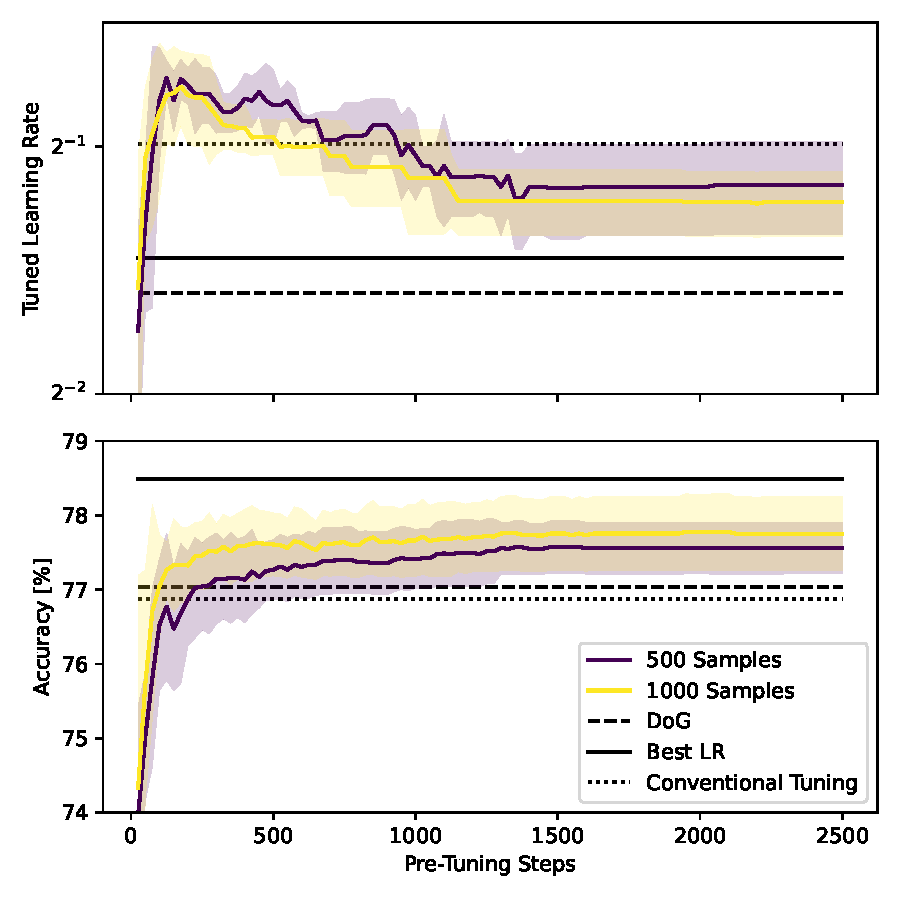
\includegraphics[width=.45\textwidth]{figures/pretune_1x64_acc_lr_exp_schedule.pdf}
	\caption{Pre-tuned LR (LR that maximizes accuracy on pre-tuning data) and resulting accuracy on data streams when using SGD and an exponential learning rate schedule with 500 or 1000 separate tuning samples. Results are averaged over all real-world datasets. The shaded area represents the 1$\sigma$-interval.}\label{fig:pretune_lr_accuracy}
\end{figure}

\begin{figure}
	\centering
	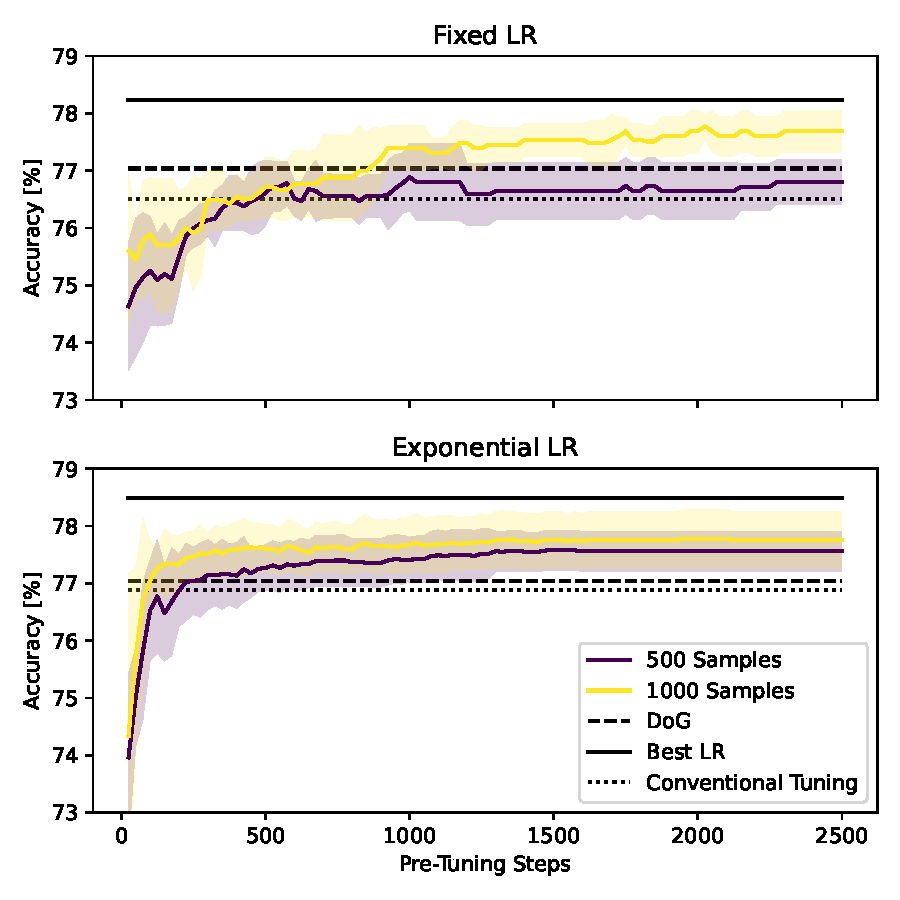
\includegraphics[width=.47\textwidth]{figures/pretune_1x64_fixed_vs_exp_schedule.pdf}
	\caption{Accuracy achieved by pre-tuning on 500 or 1000 samples when using SGD with a fixed LR schedule (top) or an exponential schedule (bottom), averaged over all real-world datasets. The shaded area represents the 1$\sigma$-interval.}\label{fig:pretune_fixed_vs_exp_lr}
\end{figure}

% \begin{figure}
% 	\centering
% 	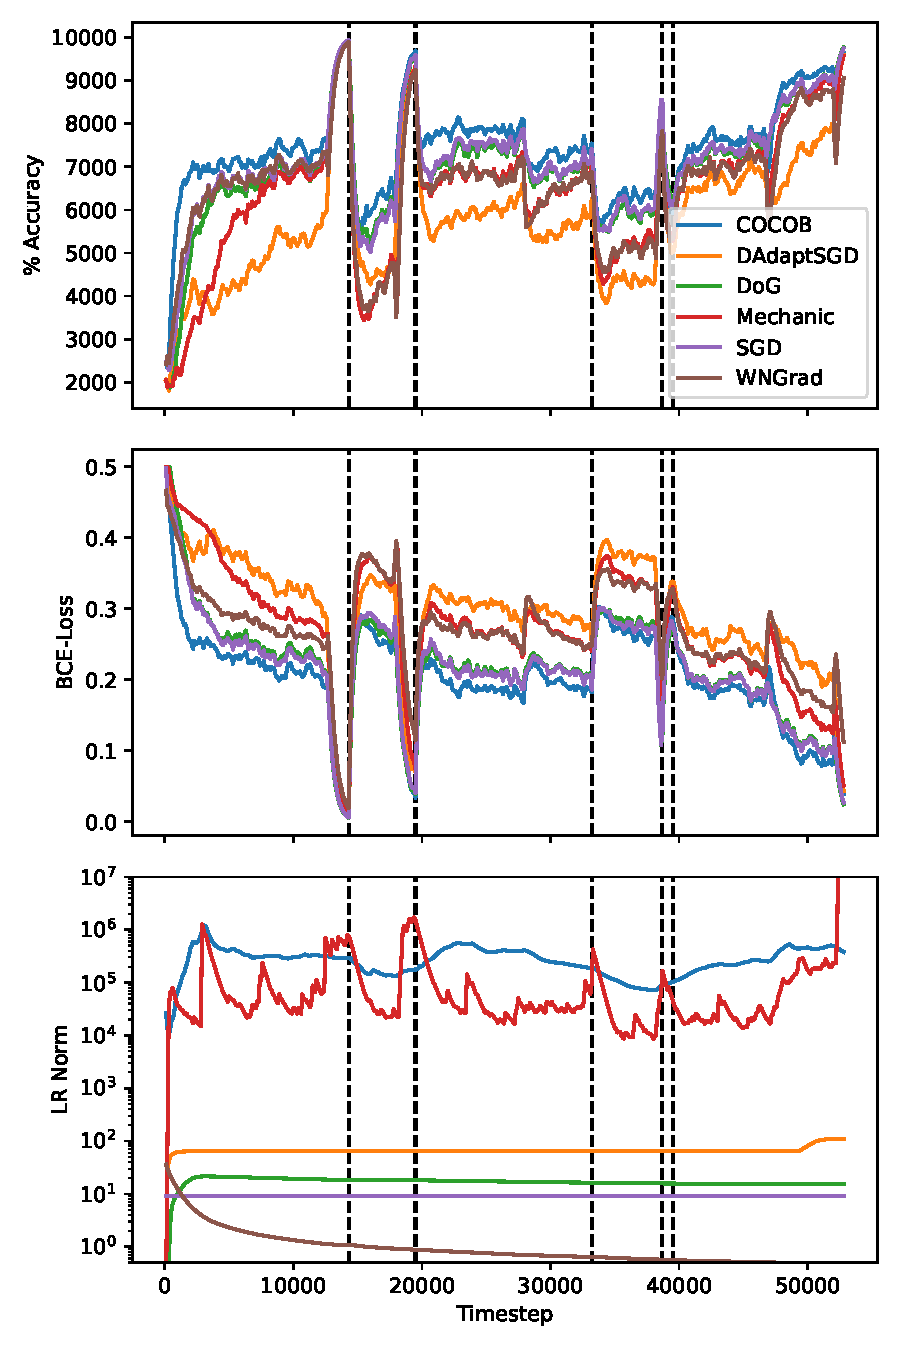
\includegraphics[width=0.47\textwidth]{figures/lr_norms_optims_insects_abrupt.pdf}
% 	\caption{Prequential accuracy, binary cross-entropy loss and LR norms $||\eta_t||$ over time for various optimization algorithms on Insects abrupt. Each dashed vertical line represents a concept drift. Lines are exponentially smoothed with a factor of 0.8.}
% \end{figure}
% \begin{figure}
% 	\centering
% 	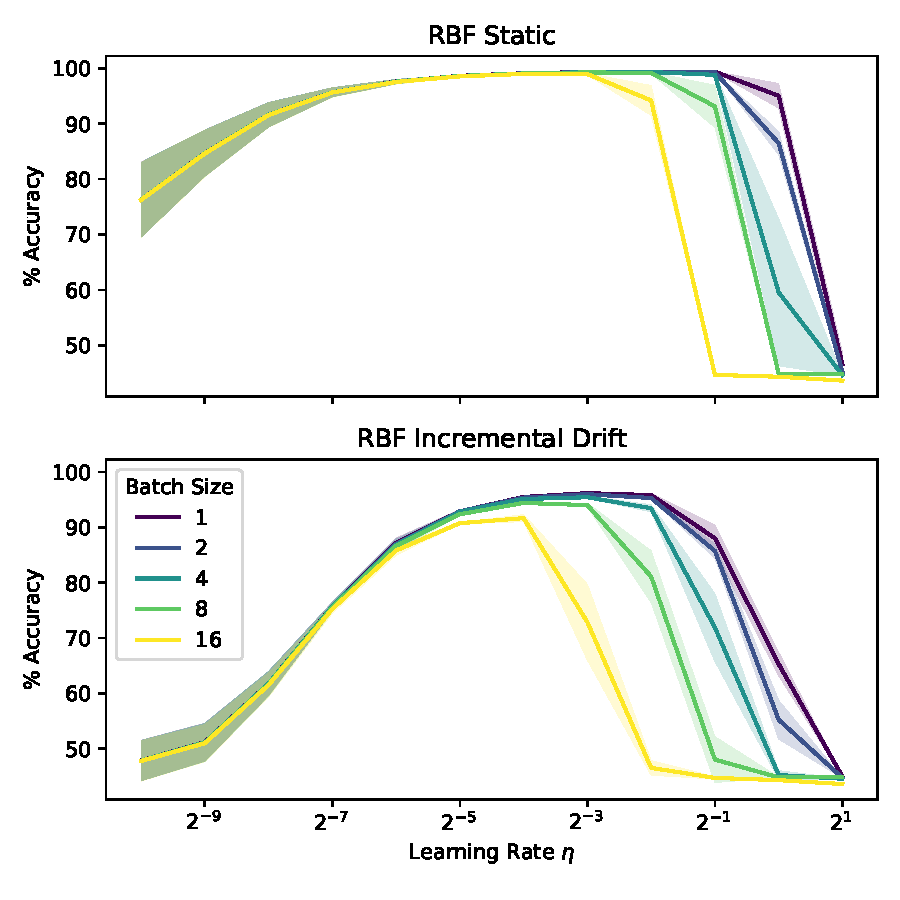
\includegraphics[width=.47\textwidth]{figures/batch_size_lr_wstd.pdf}
% 	\caption{Average accuracy over static and incrementally drifting synthetic data streams in relation to SGD mini-batch size and learning rate $\eta$. Shaded areas mark the 1$\sigma$ interval.}\label{fig:batch_size_lr}
% \end{figure}

% \begin{figure}
% 	\centering
% 	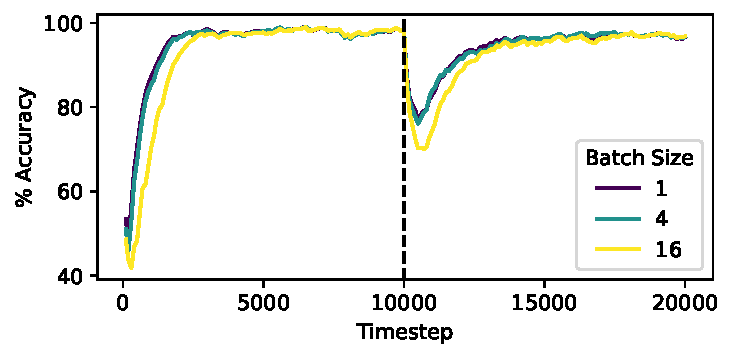
\includegraphics[width=.47\textwidth]{figures/accuracy_vs_time.pdf}
% 	\caption{Prequential accuracy for different batch sizes on RBF abrupt data stream.}
% \end{figure}

We ran prequential evaluations using basic SGD with variable batch sizes and learning rates for synthetic data streams with and without incremental concept drift, the results of which are displayed in \Cref{fig:batch_size_lr}. For static data, the average prequential accuracy over the entire stream gradually improves when moving up from an inadequately low learning rate until a certain point where training begins to diverge and performance consequently crashes. Based on our results, there seems to be an inverse relationship between batch size and both the optimal learning rate and the optimal accuracy, with larger batch sizes seemingly increasing the risk of divergence.

% The primary cause of this relationship can be seen in \Cref{fig:trajectory_batch_sizes_0.5_lr}, which depicts the trajectories of parameters of two identical MLPs trained on a bivariate data stream using batch sizes of either 4 or 16 samples. With a batch size of 16, the model has to “wait” four times longer until it receives new gradient information than the one trained with a batch size of 4. As a result, the gradient information gained from each sample on average becomes less recent and therefore less accurate with a larger batch size. Example: in \Cref{fig:trajectory_batch_sizes_0.5_lr}

\begin{equation}
\end{equation}


This effect is much stronger in the presence of concept drift as the results for RBF Incremental show.

<-could be explained by the fact that the presence of concept drift exacerbates the gradient stochasticity caused by the delay between observation and learning of samples.


\begin{figure}[ht]
	\centering
	\begin{tikzpicture}
		% Upper image
		\node[inner sep=0pt] (upper) {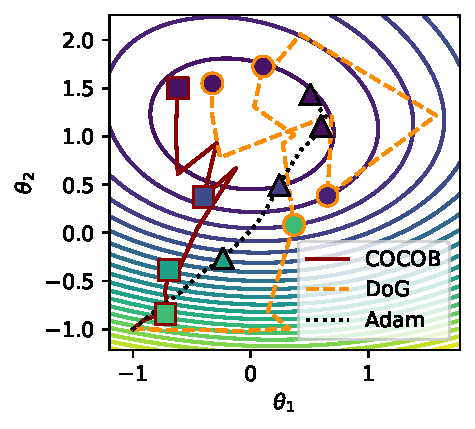
\includegraphics[width=0.4\textwidth]{figures/sgd_trajectory_optims1.pdf}};

		% Lower image
		\node[inner sep=0pt, below=3mm of upper] (lower){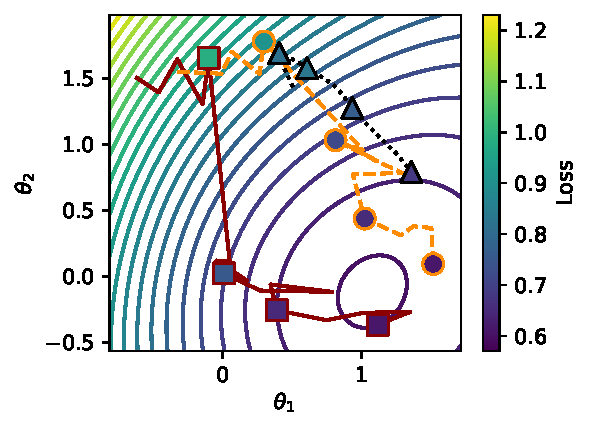
\includegraphics[width=0.4\textwidth]{figures/sgd_trajectory_optims2.pdf}};

		\path ([xshift=-8pt]upper) -- ([xshift=-8pt]lower) node[midway] (text){Concept Drift};
		\draw[->] ([xshift=-5pt, yshift=5pt]upper.south-|text.west) -- ([xshift=-5pt, yshift=-3pt]lower.north-|text.west);
		\draw[->] ([xshift=5pt, yshift=5pt]upper.south-|text.east) -- ([xshift=5pt, yshift=-3pt]lower.north-|text.east);

	\end{tikzpicture}
	\caption{Parameter trajectory of COCOB~\cite{orabonaTrainingDeepNetworks2017}, DoG~\cite{ivgiDoGSGDBest2023} and Adam~\cite{kingmaAdamMethodStochastic2017b} on synthetic data stream with abrupt concept drift. Marker colors depict the expected prequential loss over the last 16 data instances.}
\end{figure}

\section{Conclusion}


\bibliography{aaai24}

\end{document}
